\begin{frame}{$\DPLL$ алгоритмы}

    \begin{center}
        \onslide<1->{
   	\tikzstyle{vertex2} = [opacity = 0]
   	\tikzstyle{vertex3} = [opacity = 0]
    \tikzstyle{vertex4} = [opacity = 0]
   	\tikzstyle{vertex5} = [opacity = 0]
    \tikzstyle{vertex9} = [opacity = 0]
    \tikzstyle{vertex11} = [opacity = 0]
}
\only<2->{\tikzstyle{vertex2} = [opacity = 1]}
\only<3->{\tikzstyle{vertex3} = [opacity = 1]}
\only<4->{\tikzstyle{vertex4} = [opacity = 1]}
\only<5->{
  	\tikzstyle{vertex5} = [opacity = 1]
    \tikzstyle{vertex9} = [opacity = 1]
}

\tikzstyle{end} = [circle, minimum size = 0.6cm, draw = black, inner sep = 0.1pt]
            
\tikzstyle{level 1} = [draw = black, level distance = 1.5cm, sibling distance = 5cm]
\tikzstyle{level 2} = [sibling distance = 2cm]
    
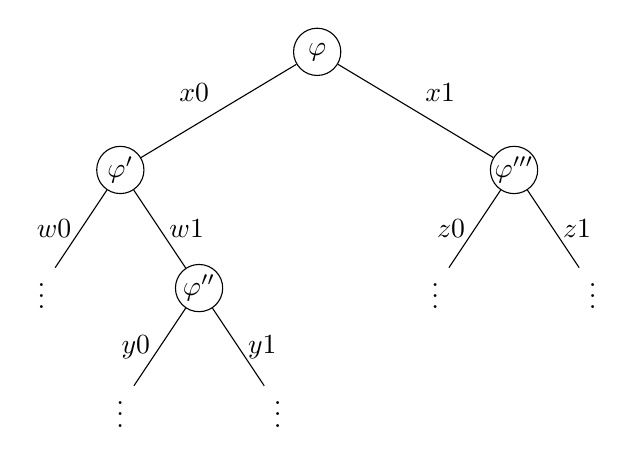
\begin{tikzpicture}[label distance=8mm]
	\node [end] (z){$\varphi$}
		child [vertex2] {
    		node [end] (b) {$\varphi'$}
			child [vertex3]{
	           	node {$\vdots$}
                edge from parent
	  	        node[left] {$w \coloneqq 0$}
            }
		    child [vertex4]{
            	node[end] {$\varphi''$}
            	child [vertex4]{
            	   	node {$\vdots$}
            		edge from parent
	  	        	node[left] {$y \coloneqq 0$}
                }
                child [vertex4]{
            	   	node {$\vdots$}
            		edge from parent
	  	        	node[right] {$y \coloneqq 1$}
            	}
                edge from parent
	   	        node[right] {$w \coloneqq 1$}
            }
           	edge from parent
            node[above left] {$x \coloneqq 0$}
        }
        child [vertex5] {
        	node [end] (c) {$\varphi'''$}
           	child [vertex9]{
               	node {$\vdots$}
                edge from parent
	            node[left] {$z \coloneqq 0$}
            }
		    child [vertex9]{
               	node {$\vdots$}
                edge from parent
	            node[right] {$z \coloneqq 1$}
            }
            edge from parent
	   	    node[above right] {$x \coloneqq 1$}
        };
\end{tikzpicture}        
    \end{center}

    
	\pause
    \pause
    \pause
    \pause
    \pause
    \begin{itemize}
        \item Эвристика $\mathbf{A}$ выбирает переменную для расщепления.
    	\pause
	    \item Эвристика $\mathbf{B}$ выбирает значения.
    	\pause
    	\item Правила упрощения: \alert{предположим, что их нет}.
    \end{itemize}
\end{frame}

\begin{frame}{$\DPLL$ и резолюция}
    
    \begin{theorem}
        $\DPLL$ алгоритм делает $t$ расщеплений на невыполнимой формуле
        $$\varphi \coloneqq \bigvee\limits_i C_i$$
        $\Rightarrow$ существует резолюционное доказательство $\varphi$ размера $2t$.
    \end{theorem}

    \pause

    \begin{minipage}{0.58\linewidth}
        \centering
        \tikzstyle{inner} = [circle, minimum size = 0.3cm, draw, inner sep = 0.1pt]
\tikzstyle{gstyle} = [fill = green]
\tikzstyle{rstyle} = [fill = red]
\tikzstyle{ed} = [->, draw]
\tikzstyle{ops} = [alt=<{#1-}>{opacity = 1}{opacity = 0}]
\tikzstyle{opstyle} = [inner, ops = #1]
\tikzstyle{oped} = [ed, ops = #1]
\tikzstyle{gstyle} = [alt=<{#1}>{fill = green}{}]
\tikzstyle{rstyle} = [alt=<{#1}>{red!90!black}{}]
\tikzstyle{snakestyle} = [
    alt=<{#1}>{
        decorate,
        decoration = {
            snake,
            amplitude = 0.4mm,
            segment length = 2mm,
            post length = 1mm
        }
    }{}]


    
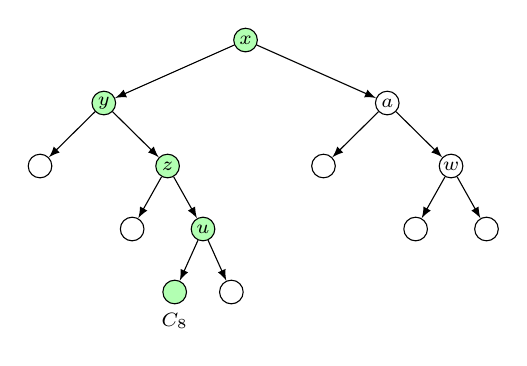
\begin{tikzpicture}[>=latex, xscale = 0.9]
    
    \node[inner, fill = green!30] (a) at (0, 0) {\scriptsize $x$};
    \node[inner, fill = green!30] (b) at (-2, -0.8) {\scriptsize $y$};
    \node[inner] (c) at (2, -0.8) {\scriptsize $a$};
    \node[inner] (d) at (-2.9, -1.6) {};
    \node[inner, fill = green!30] (e) at (-1.1, -1.6) {\scriptsize $z$};
    \node[inner] (f) at (1.1, -1.6) {};
    \node[inner] (g) at (2.9, -1.6) {\scriptsize $w$};

    \node[inner] (h) at (-1.6, -2.4) {};
	\node[inner, fill = green!30] (i) at (-0.6, -2.4) {\scriptsize $u$};
    
    \node[inner] (j) at (2.4, -2.4) {};
    \node[inner] (k) at (3.4, -2.4) {};

    \node[inner, fill = green!30] (l) at (-1, -3.2) {};
    \node[below = 4pt] at (l) {\scriptsize $C_{8}$};
    \node[inner] (m) at (-0.2, -3.2) {};
    
    \draw[ed] (a) -- (b);
    \draw[ed] (a) -- (c);
    \draw[ed] (b) -- (d);
    \draw[ed] (b) -- (e);
    \draw[ed] (c) -- (f);
    \draw[ed] (c) -- (g);
    \draw[ed] (e) -- (h);
    \draw[ed] (e) -- (i);
    \draw[ed] (g) -- (j);
    \draw[ed] (g) -- (k);
    \draw[ed] (i) -- (l);
    \draw[ed] (i) -- (m);
\end{tikzpicture}
    \end{minipage}
    \pause
    \begin{minipage}{0.4\linewidth}
        \centering
        $\frac{A \lor x ~~~ B \lor \neg x}{A \lor B} ~~~~~ \frac{A}{A \lor z}$
        \begin{itemize}
            \item Вершина $\Rightarrow$ дизъюнкция отрациний запросов.
            \item $(x \lor \neg y \lor \neg z \lor u)$.
        \end{itemize}
    \end{minipage}

\end{frame}


\begin{frame}{Pigeonhole Principle и $\DPLL$ алгоритмы}

    Переменные: $x_{i, j}$, $i \in \{1, 2, \dots, n + 1\}$, $j \in \{1, 2, \dots, n\}$.
    \vspace{0.1cm}

    \pause
    \begin{itemize}
        \item $\bigvee\limits_{j = 1}^{n} x_{i, j}$;
        \item $\neg x_{i, j} \lor \neg x_{i', j}$.
    \end{itemize}

    \pause

    \vspace{0.2cm}
    \begin{minipage}{0.3\linewidth}
        \centering
        \tikzstyle{undir} = [thick]
\tikzstyle{dir} = [thick, ->, bend left = 12]
\tikzstyle{ver} = [thick, ->, draw, circle]

\begin{tikzpicture}[black, >=stealth']

    \node[ver] (A) at (0, 0) {};
    \node[ver] (B) at (2, 2) {};
    \node[ver] (C) at (3, 0) {};
    \node[ver] (D) at (4, 1) {};
    \node[ver] (E) at (3.5, 3.5) {};
    \node[ver] (F) at (-0.5, 3) {};

    \only<1>{
        \draw[undir] (A) to (B);
        \draw[undir] (A) to (C);
        \draw[undir] (B) to (C);
        \draw[undir] (C) to (D);
        \draw[undir] (B) to (D);
        \draw[undir] (D) to (E);
        \draw[undir] (E) to (F);
        \draw[undir] (F) to (A);
        \draw[undir] (B) to (F);
    }
    
	\only<2->{
        \draw[dir] (A) to (B);
        \draw[dir] (A) to (C);
        \draw[dir] (B) to (C);
        \draw[dir] (C) to (D);
        \draw[dir] (B) to (D);
        \draw[dir] (D) to (E);
        \draw[dir] (E) to (F);
        \draw[dir] (F) to (A);
        \draw[dir] (B) to (F);

        \draw[dir] (B) to (A);
        \draw[dir] (C) to (A);
        \draw[dir] (C) to (B);
        \draw[dir] (D) to (C);
        \draw[dir] (D) to (B);
        \draw[dir] (E) to (D);
        \draw[dir] (F) to (E);
        \draw[dir] (A) to (F);
        \draw[dir] (F) to (B);
    }
\end{tikzpicture}

    \end{minipage}
    \pause
    \begin{minipage}{0.68\linewidth}
        \centering
        \includegraphics[width = 0.3\textwidth]{pics/pigeon3.png}
        \pause
        \begin{theorem}[Haken 85]
            Любое резолюционное доказтельство данной формулы имеет размер $2^{\Omega(n)}$.
        \end{theorem}
    \end{minipage}
    
\end{frame}
